\documentclass[12pt]{article}

\usepackage{amsmath}
\usepackage{graphicx}
\usepackage{hyperref}
\usepackage[letterpaper,top=2cm,bottom=2cm,left=3cm,right=3cm]{geometry}
\usepackage{subfig}

\title{Springed Cart and Pendulum Report}
\author{Next Ongarjvaja and Will Hodges}
\date{Fall 2024}

\begin{document}

\maketitle

\section{Introduction}

In our project, we studied the cart on a spring system. The system consists of a cart being driven by a spring, with a pendulum attached to the cart, shown in \autoref{fig:diagram}. To analyze this system, we derived and simplified the equations of motion using Lagrangian mechanics. We then numerically solved these equations using Python in order to understand the motion of the system for various parameters and initial conditions. An animation showing the results of one of our solutions can be found \href{https://github.com/NextZtepS/SpringedCart_and_Pendulum/blob/main/animation.gif}{here}. We found that there are two modes that describe the motion of the system—the pendulum mode and the cart mode. We found solutions where one of these modes dominated over the other, and also solutions where these modes were comparable.

\begin{figure}
    \centering
    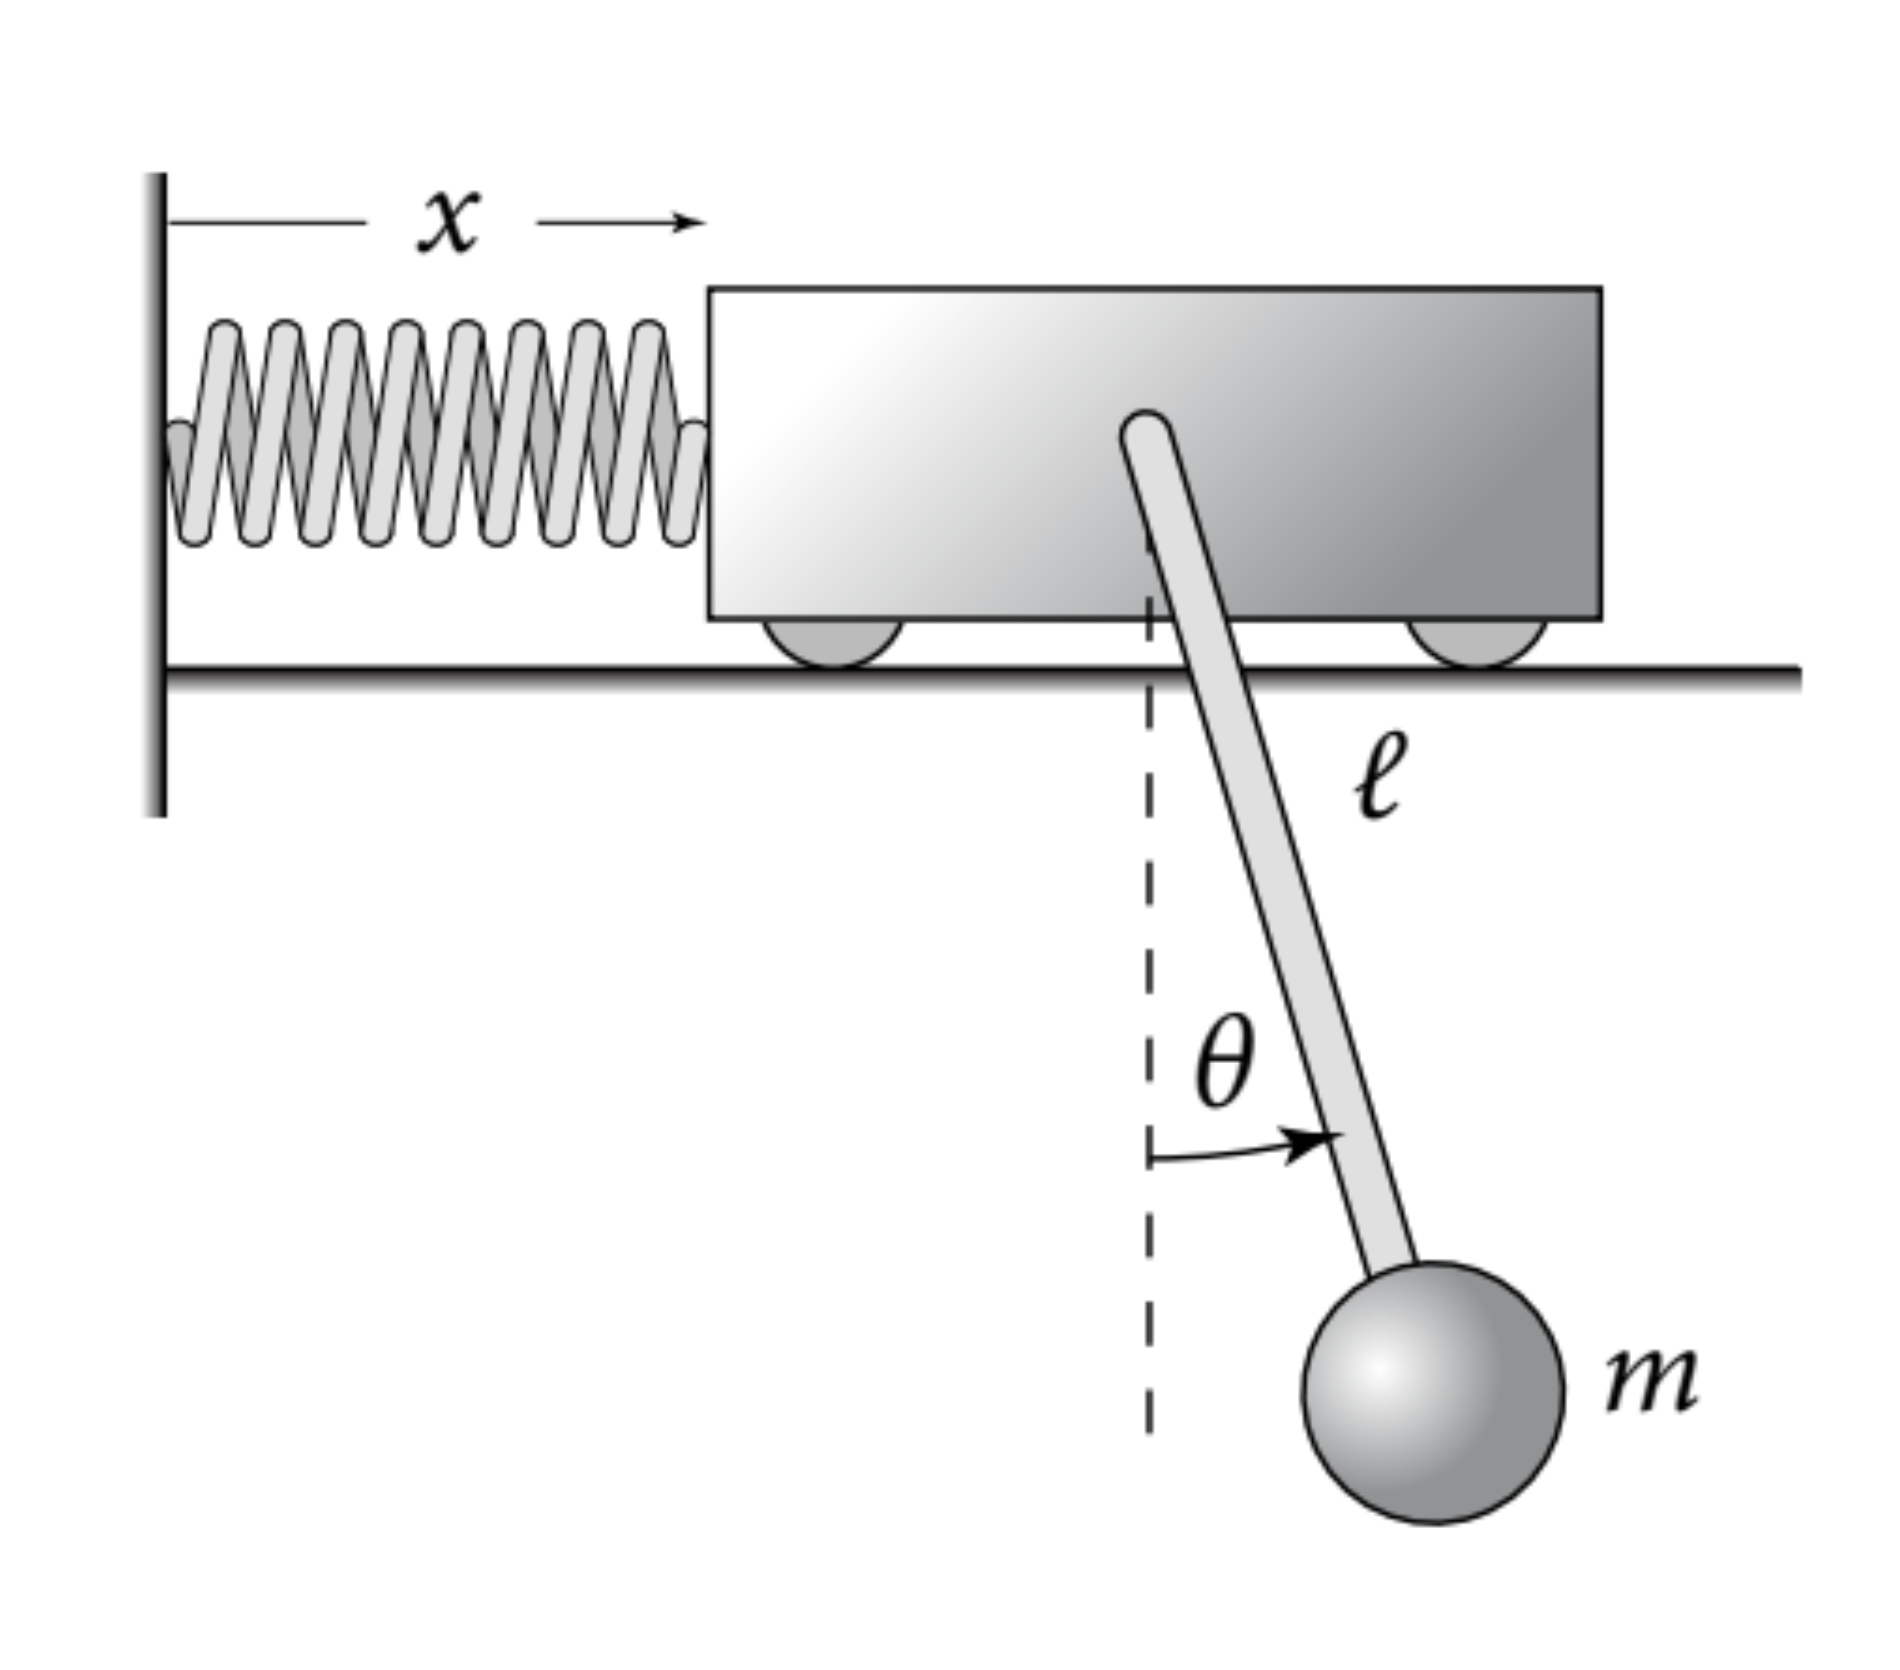
\includegraphics[width=0.5\textwidth]{figures/diagram.png}
    \caption{\small{Cart on a spring system. In the system, a cart of mass $M$ rolls on a frictionless horizontal surface. The cart is attached to a massless spring of force constant $k$ and equilibrium length $d$, which is attached to a wall on the left. The distance between the left end of the cart and the wall is $x$. A pendulum of mass $m$ and length $l$ hangs from the cart. The pendulum is restricted to the vertical plane, and swings at angle $\theta$ to the vertical. Figure taken from project ideas handout.}}
    \label{fig:diagram}
\end{figure}

\section{Theoretical Analysis}
\subsection{The Lagrangian}

Referring back to the \autoref{fig:diagram}, we first describe the position of the cart using $\Vec{r_M}$ and that of the pendulum using $\Vec{r_m}$ in the Cartesian basis for convenient Lagrangian calculation. We will later describe the system in terms of the non-dimensionalized length $x$, angle $\theta$, and time $t$. Note that the position of the pendulum depends on the that of the cart which we organize into the two equations below.
\begin{align}
	\Vec{r_M} &= x \hat{x} \label{eq:r_M} \\
    \Vec{r_m} &= (x + l\sin{\theta}) \hat{x} + (-l\cos{\theta}) \hat{y} \label{eq:r_m}
\end{align}

Then, we come up with the equations for the kinetic and potential energy of the two masses as follows.

\begin{align}
	U &= U_{spring} + U_{gravity} = \frac{1}{2}k(x-d)^2 + (-mgl\cos{\theta})
      \label{eq:U} \\
    T &= T_{cart} + T_{pendulum} = \frac{1}{2}M(\dot{\Vec{r_M}})^2 + \frac{1}{2}m(\dot{\Vec{r_m}})^2 = \frac{1}{2} \big[ (M+m)\dot{x}^2 + m(l^2\dot{\theta}^2 + 2l\dot{x}\dot{\theta}\cos{\theta}) \big] \label{eq:T}
\end{align}

Finally, the Lagrangian of the system can be computed as follows.

\begin{align}
    L &= T - U = \frac{1}{2} \big[ (M+m)\dot{x}^2 + ml^2\dot{\theta}^2 + 2ml\cos{\theta}\dot{x}\dot{\theta}\big] - \frac{1}{2} \big[ k(x-d)^2 - 2mgl\cos{\theta} \big] \label{eq:L}
\end{align}

\subsection{Equations of Motion}

After obtaining the Lagrangian, we compute the Euler-Lagrange equations (equations of motion) for the two generalized coordinates $x$ and $\theta$ using the relationship $\frac{d}{dt} (\frac{\partial L}{\partial \dot{p}}) = \frac{\partial L}{\partial p}$ where $p$ is a generalized coordinate. For the $x$ coordinate, we have the equation that follows.

\begin{align}
        \frac{d}{dt} (\frac{\partial L}{\partial \dot{x}}) &= \frac{\partial L}{\partial x} \\
    (M+m)\Ddot{x} + ml\cos{\theta}\Ddot{\theta} - ml\sin{\theta}\dot{\theta}^2 &= 
     -k(x-d) \label{eq:x}
\end{align}
     
And we continue the same derivation for the $\theta$ coordinate to get

\begin{align}
    \frac{d}{dt} (\frac{\partial L}{\partial \dot{\theta}}) &= \frac{\partial L}{\partial \theta} \\
    ml^2\Ddot{\theta}^2 + ml\cos{\theta} &= -mgl\sin{\theta} \label{eq:theta}.
\end{align}

Normally, we can numerically solve the two differential equations above with various initial conditions already. However, we choose to non-dimensionalize the equations allowing for a more convenient analysis with different physical parameters by defining a non-dimensionalized time and length as follows.

\begin{align}
    \tau &= \frac{t}{T} \label{eq:tau} \\
    X &= \frac{x-d}{L} \label{eq:X}
\end{align}

From this, we have that $\frac{d}{dt} = \frac{1}{T} \frac{d}{d\tau}$ and $\frac{d^2}{dt^2} = \frac{1}{T^2} \frac{d^2}{d\tau^2}$. Then, we substitute these into \autoref{eq:x} and \autoref{eq:theta} to get the non-dimensionalized version as follows.

\begin{align}
    \frac{d^2X}{d\tau^2} &= \frac{1}{(M+m)L} \big[ -ml\cos{\theta} \frac{d^2\theta}{d\tau^2} + ml\sin{\theta}(\frac{d\theta}{d\tau})^2 - kLT^2X \big] \label{eq:nond_X} \\
    \frac{d^2\theta}{d\tau^2} &= \frac{1}{l} \big[ -L\cos{\theta}\frac{d^2X}{d\tau^2} - gT^2\sin{\theta} \big] \label{eq:nond_theta}
\end{align}

In the next section, we numerically solve the two non-dimensionalized differential equations to observe some interesting results.

\section{Numerical Analysis}

We numerically solved the system by varying the parameters involved. The three main system parameters that we are interested in include: 1) the ratio between mass of cart and mass of the pendulum $r_{mass}$ 2) the natural frequency of the mass-spring system $f_{msp}$ 3) the natural angular of the pendulum $f_{pen}$. We define the three parameters as follows.

\begin{align}
    r_{mass} &= \frac{M}{m} \\
    f_{msp} &= \frac{1}{2\pi}\sqrt{\frac{k}{M+m}} \\
    f_{pen} &= \frac{1}{2\pi}\sqrt{\frac{g}{l}}
\end{align}

As for other parameters, we keep the length of pendulum $l = 1$ m, unit time $T = 1$, and unit length $L = 1$. In the following sections, we analyze different cases of $f_{msp}$ and $f_{pen}$ where the mass ratio $r_{mass}$ is represented by 3 ratios of 0.1, 1, and 10 in which the total mass is equal to 1 in all ratios.

\subsection{Pendulum-mode Motion}

We first investigated the case where the natural frequency of the pendulum is much greater then the natural frequency of the mass spring system, shown in \autoref{fig:pendulum-mode}. In this case, the pendulum mode and its motion dominates the system. This results in simple pendulum motion, and chaotic motion for the mass spring system. In the state space plots, we can see that the pendulum's motion repeats every cycle, whereas the cart's motion is complex.

Since the natural frequency of the pendulum is much greater than the natural frequency of the mass spring system, the pendulum will have more energy then the cart. This means that the motion of the pendulum can overpower the motion of the cart. Since our gravity is extremely high in this example, we see that the pendulum never flips over, which would appear as a horizontal line across the plot. Also, as the mass ratio decreases, we see that the transition between potential energy to kinetic energy of the pendulum becomes more pronounced as its being pulled more strongly by the gravitational force. We also noticed that the cart's motion seems to be periodic over a long timescale.

\begin{figure}
    \centering
    \subfloat{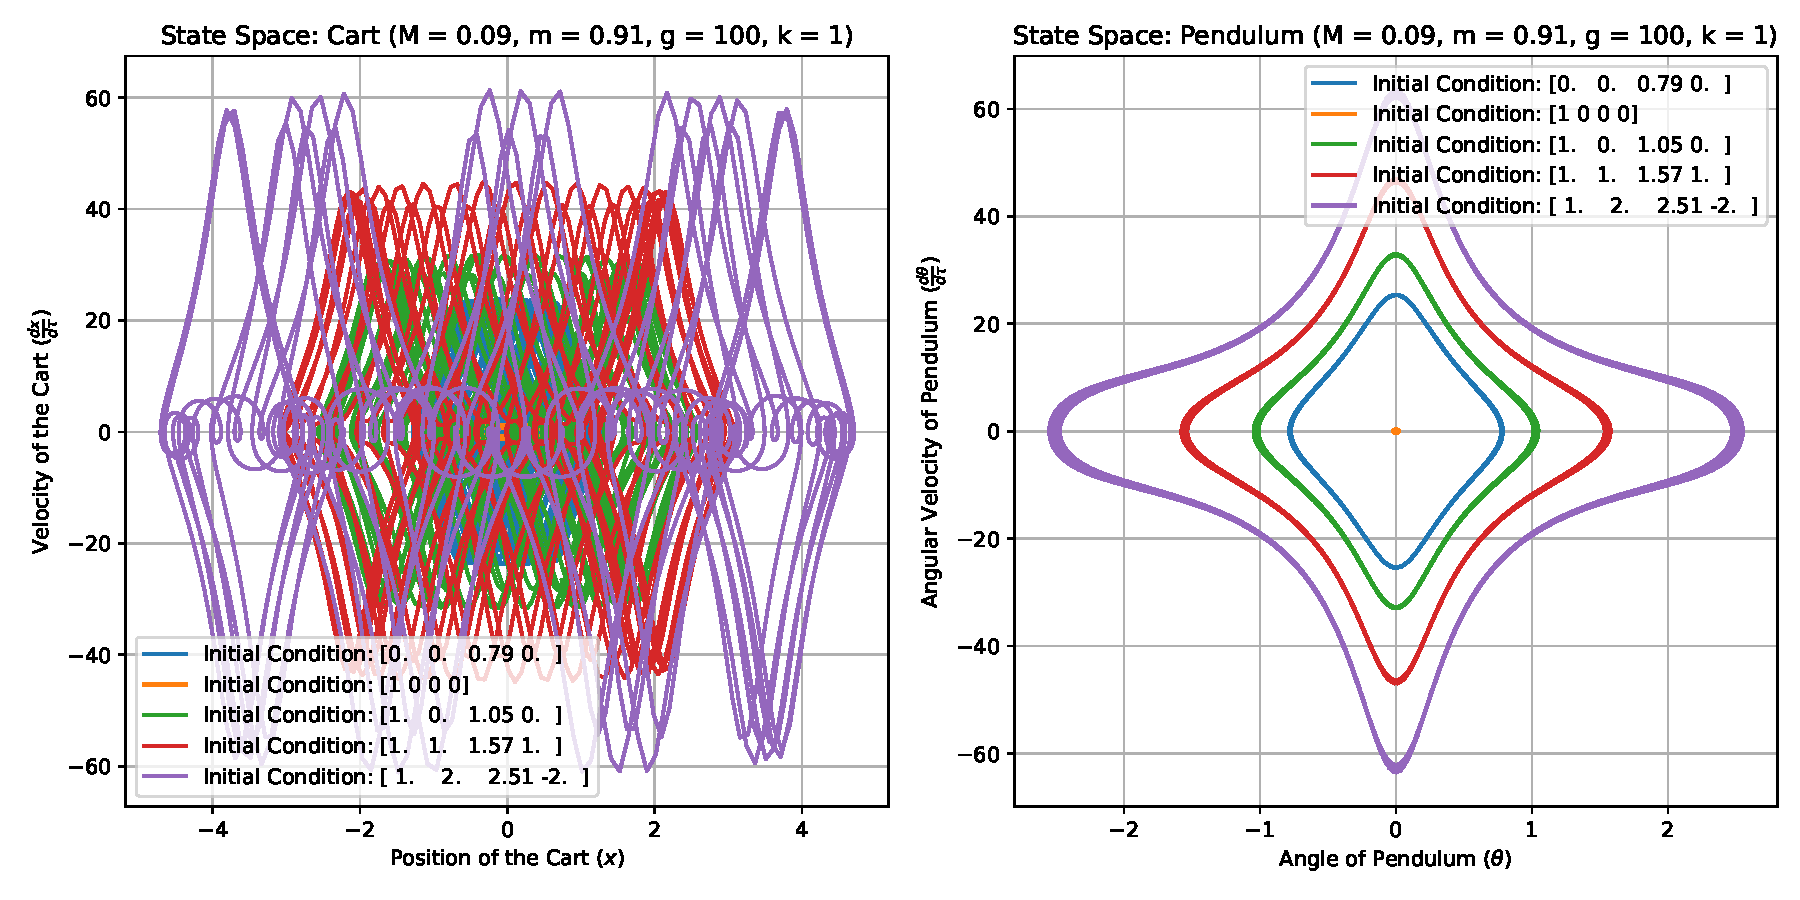
\includegraphics[width=0.9\textwidth]{figures/r-0-k-1-g-100.pdf}} \\
    \subfloat{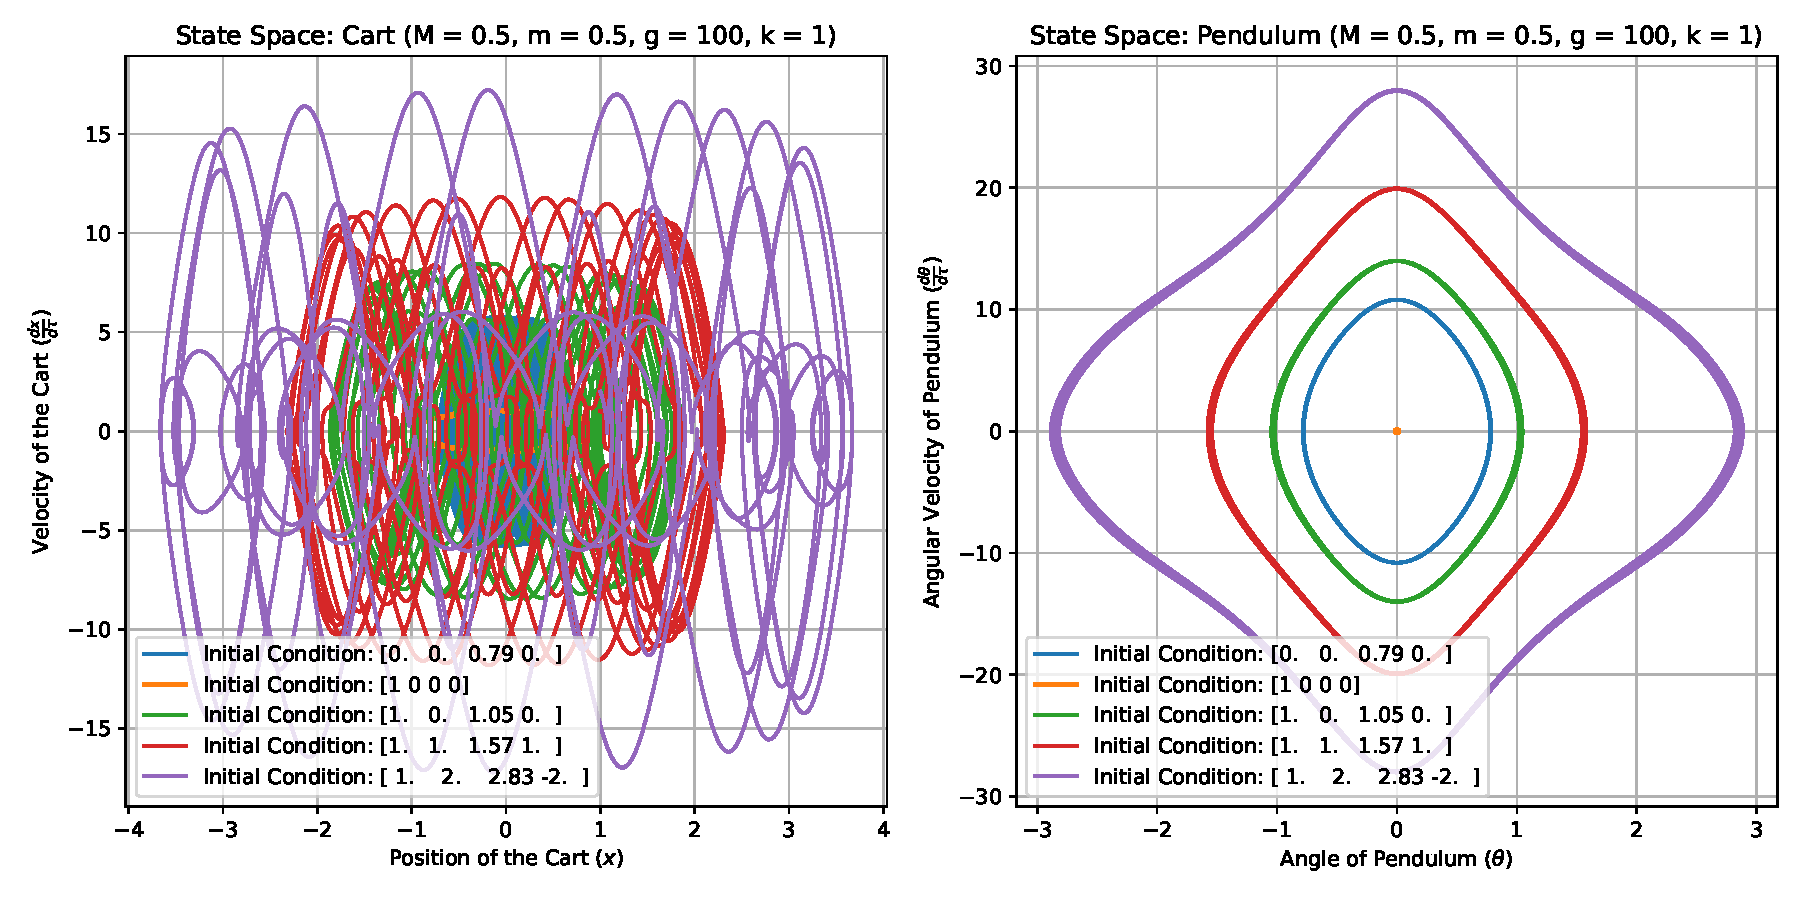
\includegraphics[width=0.9\textwidth]{figures/r-1-k-1-g-100.pdf}} \\
    \subfloat{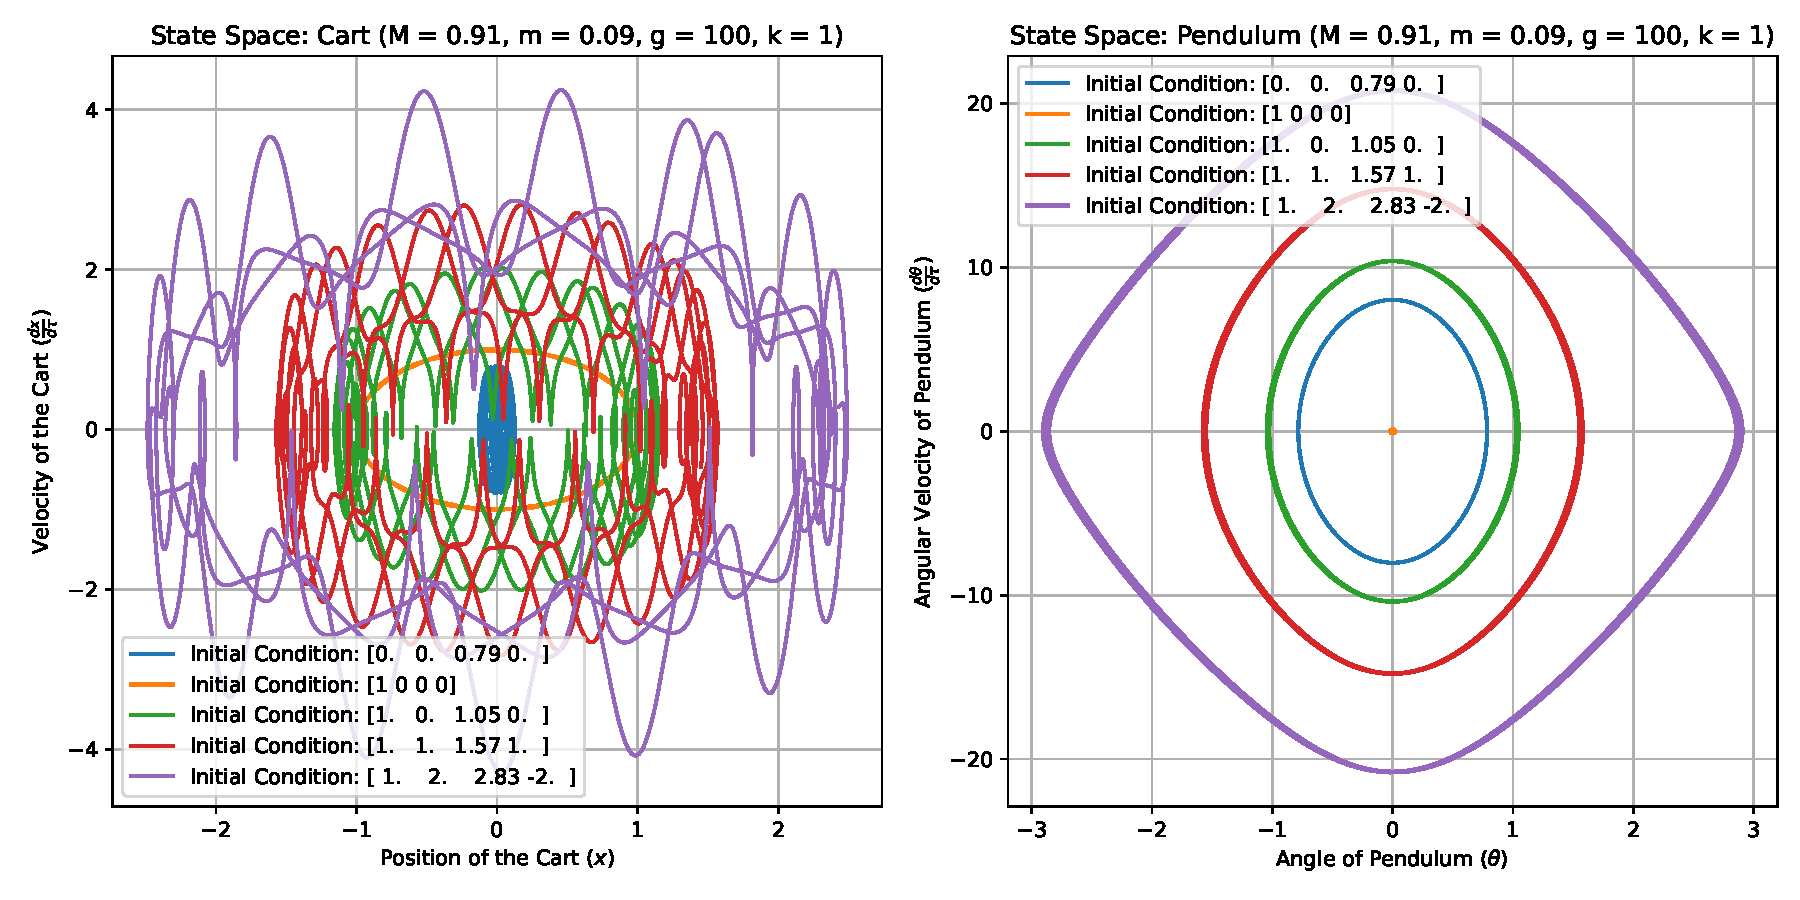
\includegraphics[width=0.9\textwidth]{figures/r-10-k-1-g-100.pdf}}
    \caption{\small{Series of state space plots where $f_{msp} \ll \ f_{pen}$ ($g$ = 100, $k$ = 1). From top to bottom, the rows illustrate the mass ratios 0.1, 1, and 10. On the left is the state space of $X$ and that of $\theta$ on the right. The initial conditions are ordered as $[X_0, \frac{dX}{d\tau}_0, \theta_0, \frac{d\theta}{d\tau}_0]$.}}
    \label{fig:pendulum-mode}
\end{figure}

\subsection{Cart-mode Motion}

Secondly, we investigated the case where the natural frequency of the mass spring is much greater then the natural frequency of the pendulum, shown in \autoref{fig:cart-mode}. In this case, the mass spring system mode and its motion dominates the system. This results in a near simple harmonic motion on the mass spring system, and chaotic motion for the pendulum. In the state space plots, we can see that the cart's motion is bound within the circular envelope, which represents the case of pure simple harmonic motion, and being regularly disturbed by the the chaotic motion of the pendulum. 

Since the natural frequency of the mass spring system is much greater than the natural frequency of the pendulum, the mass spring system will have more energy than the pendulum. This means that the regular motion of the cart is constantly pushed around by the pendulum. As the mass ratio increases, the motion of the cart becomes more regular and resembles the simple harmonic case. This is because the influence of the pendulum's motion is minimized by its decreasing mass. Also, we observe that the pendulum is being driven by the energy stored in the spring causing it to flip over in a chaotic manner. One special case is when the system starts off at rest with the spring unstretched where the pendulum angle is the only source of energy; since the spring is very stiff, the cart's motion is minimized and the overall motion simplifies to a simple pendulum instead.

\begin{figure}
    \centering
    \subfloat{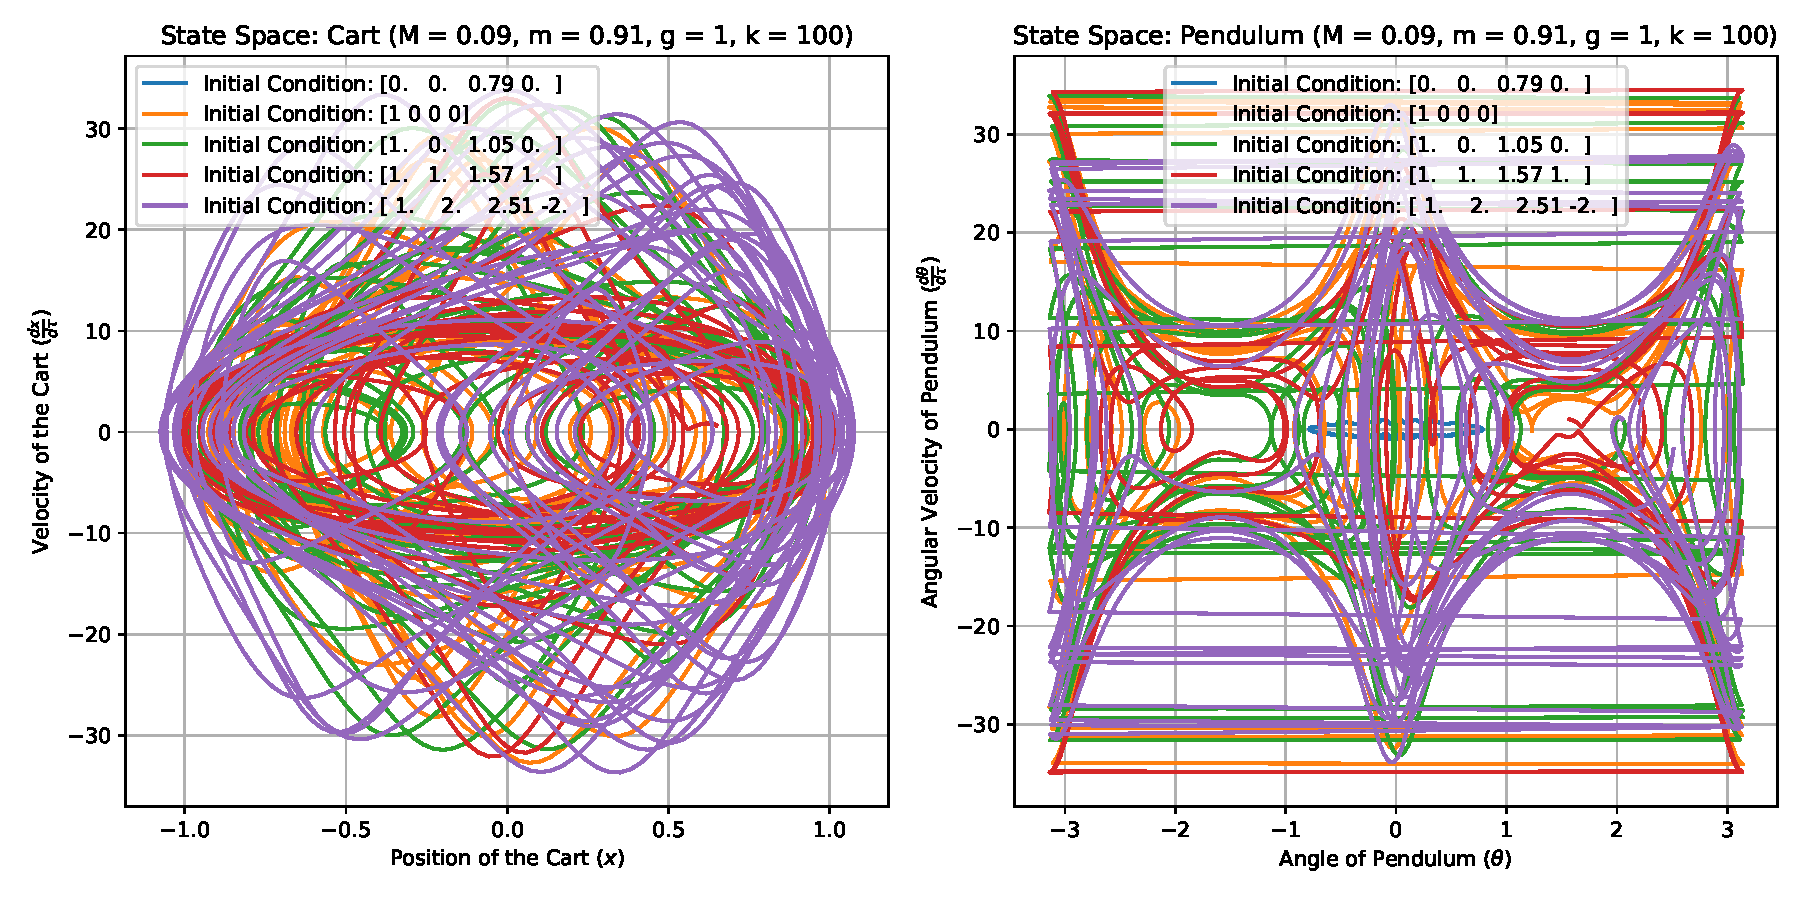
\includegraphics[width=0.9\textwidth]{figures/r-0-k-100-g-1.pdf}} \\
    \subfloat{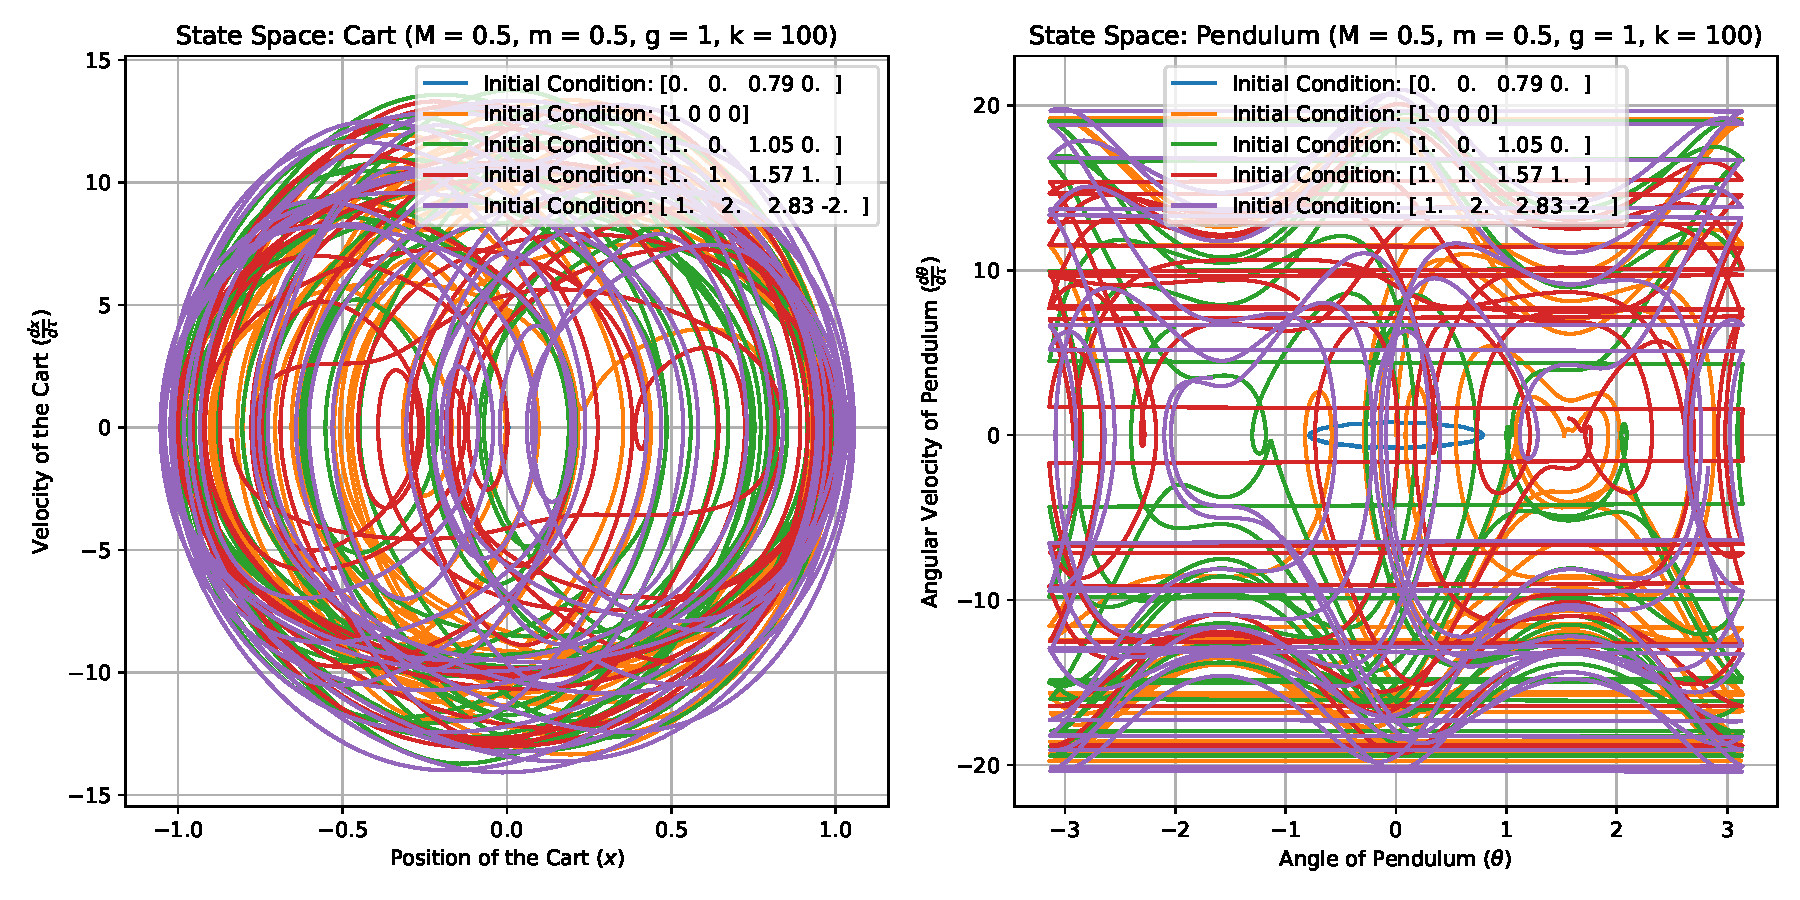
\includegraphics[width=0.9\textwidth]{figures/r-1-k-100-g-1.pdf}} \\
    \subfloat{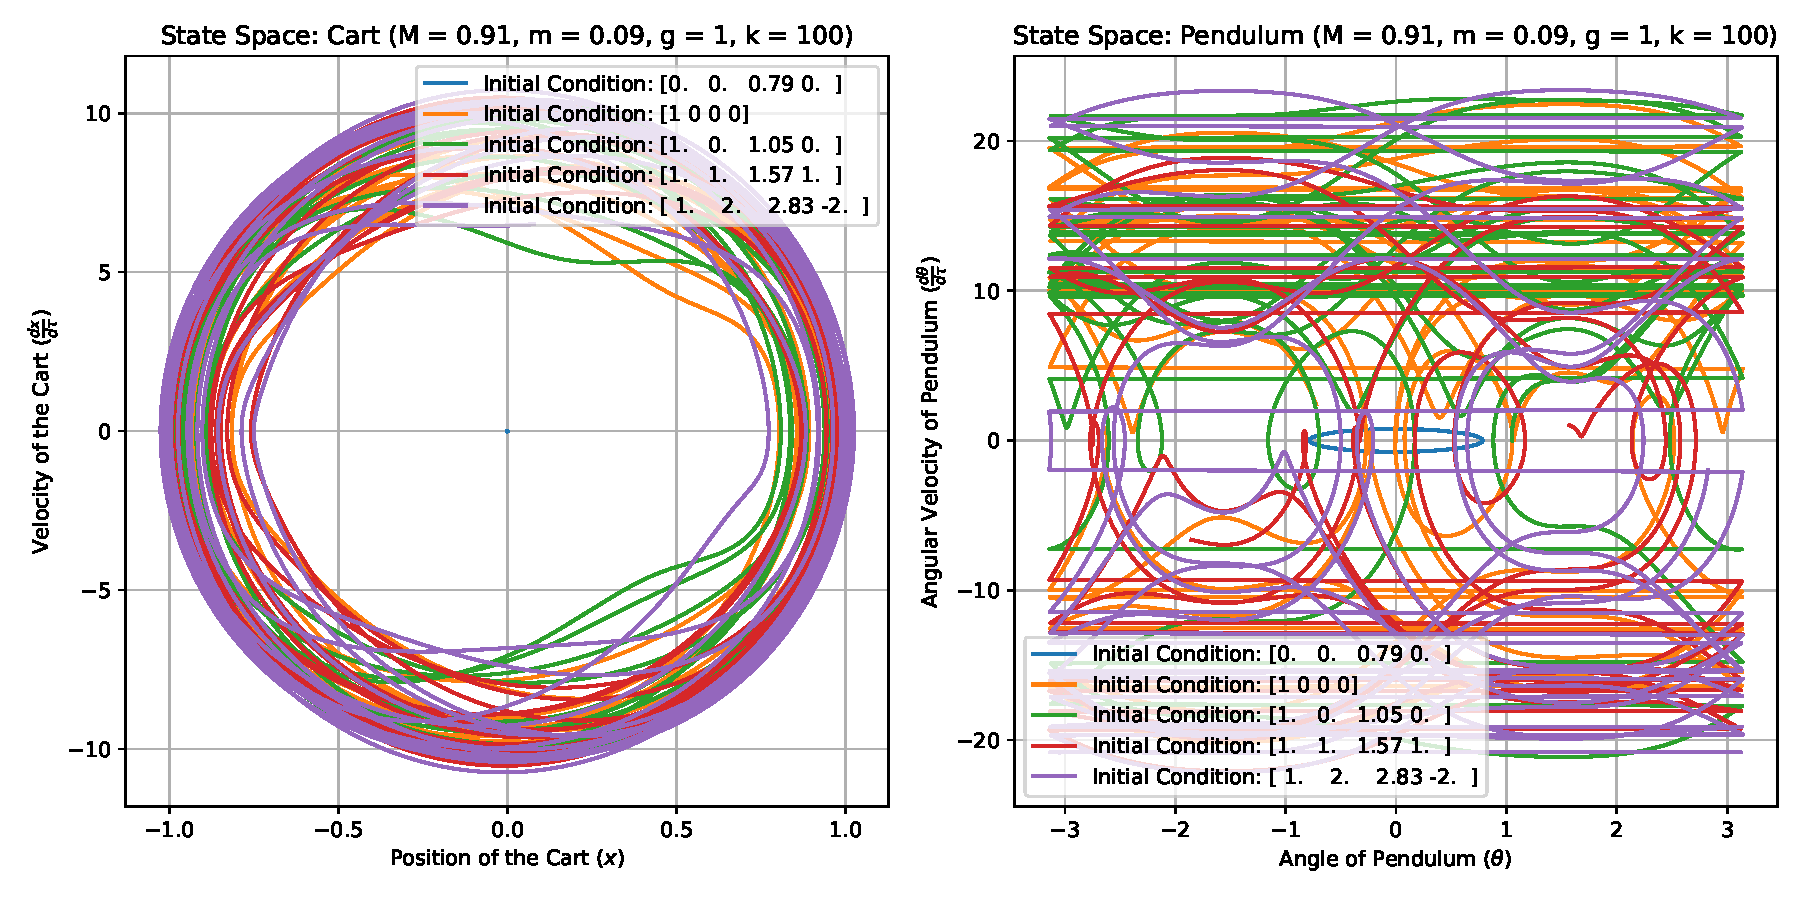
\includegraphics[width=0.9\textwidth]{figures/r-10-k-100-g-1.pdf}}
    \caption{\small{Series of state space plots where $f_{msp} \gg \ f_{pen}$ ($g$ = 1, $k$ = 100). From top to bottom, the rows illustrate the mass ratios 0.1, 1, and 10. On the left is the state space of $X$ and that of $\theta$ on the right. The initial conditions are ordered as $[X_0, \frac{dX}{d\tau}_0, \theta_0, \frac{d\theta}{d\tau}_0]$.}}
    \label{fig:cart-mode}
\end{figure}

\subsection{Mixed-mode Motion}

Finally, we investigated the case where the natural frequency of the pendulum is equal to the natural frequency of the mass spring system, shown in \autoref{fig:mixed-mode}. In this case, the motion of both the mass spring system and pendulum is mostly chaotic. Since the energies of the systems are comparable, the motions are able to significantly affect each other. However, in the case where the mass of the cart is much greater then the mass of the pendulum, we can see that the cart starts to display a more stable simple harmonic motion. This is likely due to the cart gaining energy relative to the pendulum due to its increased mass.

\begin{figure}
    \centering
    \subfloat{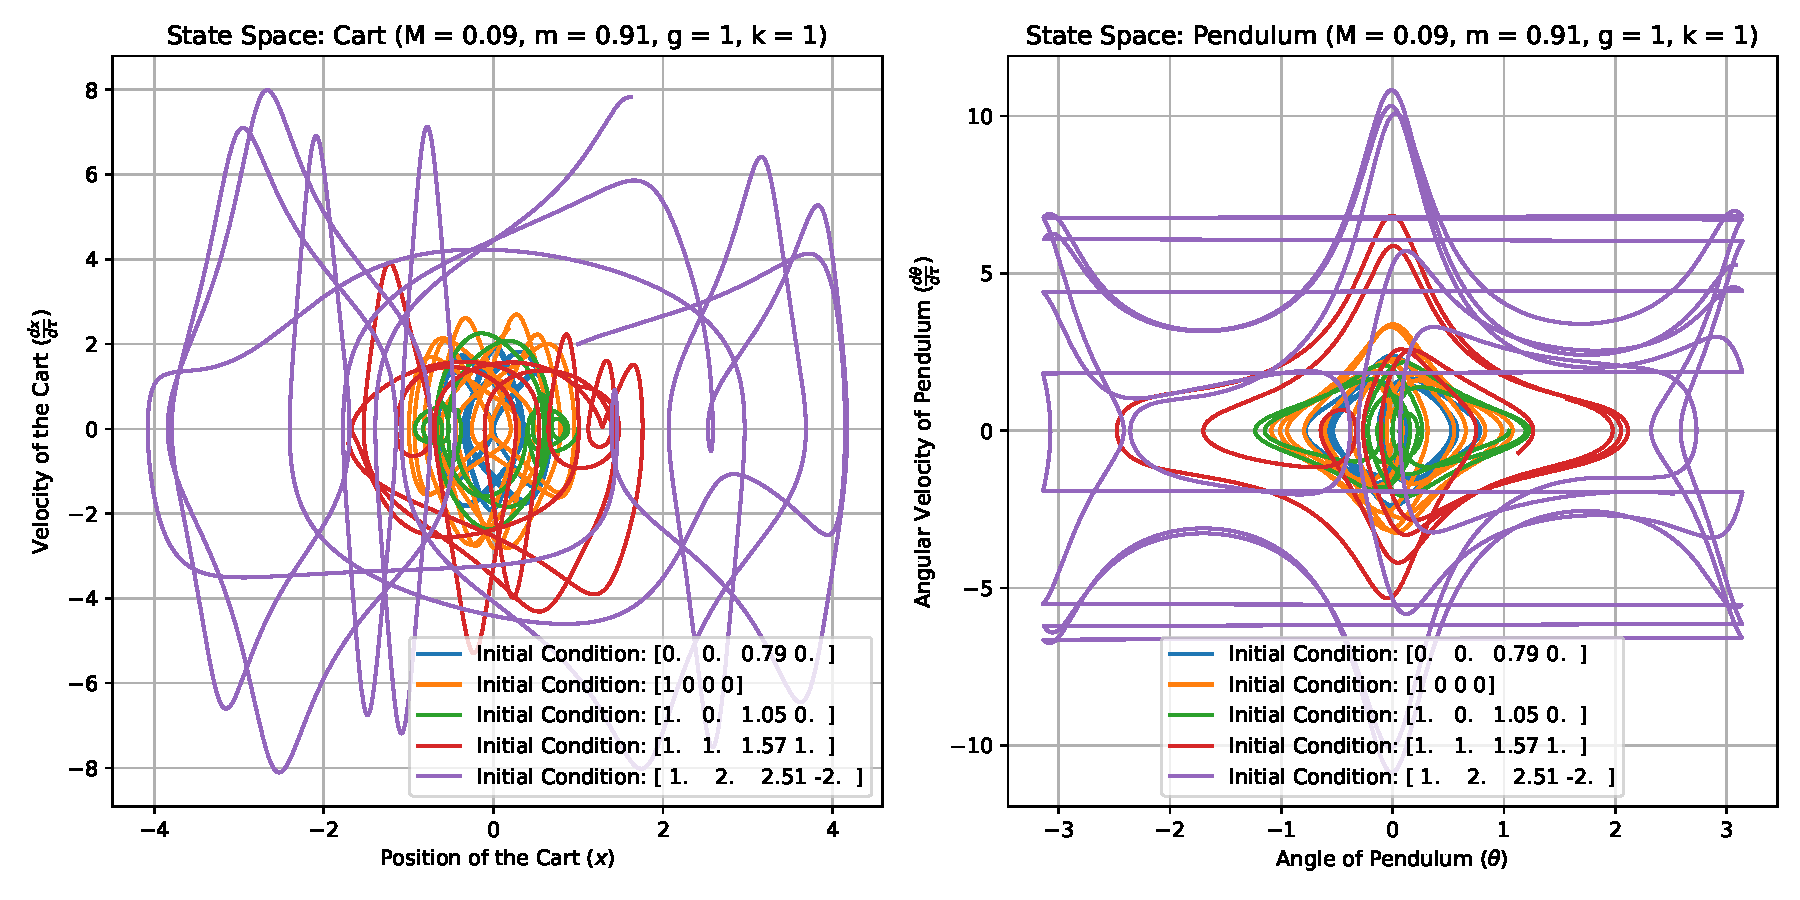
\includegraphics[width=0.9\textwidth]{figures/r-0-k-1-g-1.pdf}} \\
    \subfloat{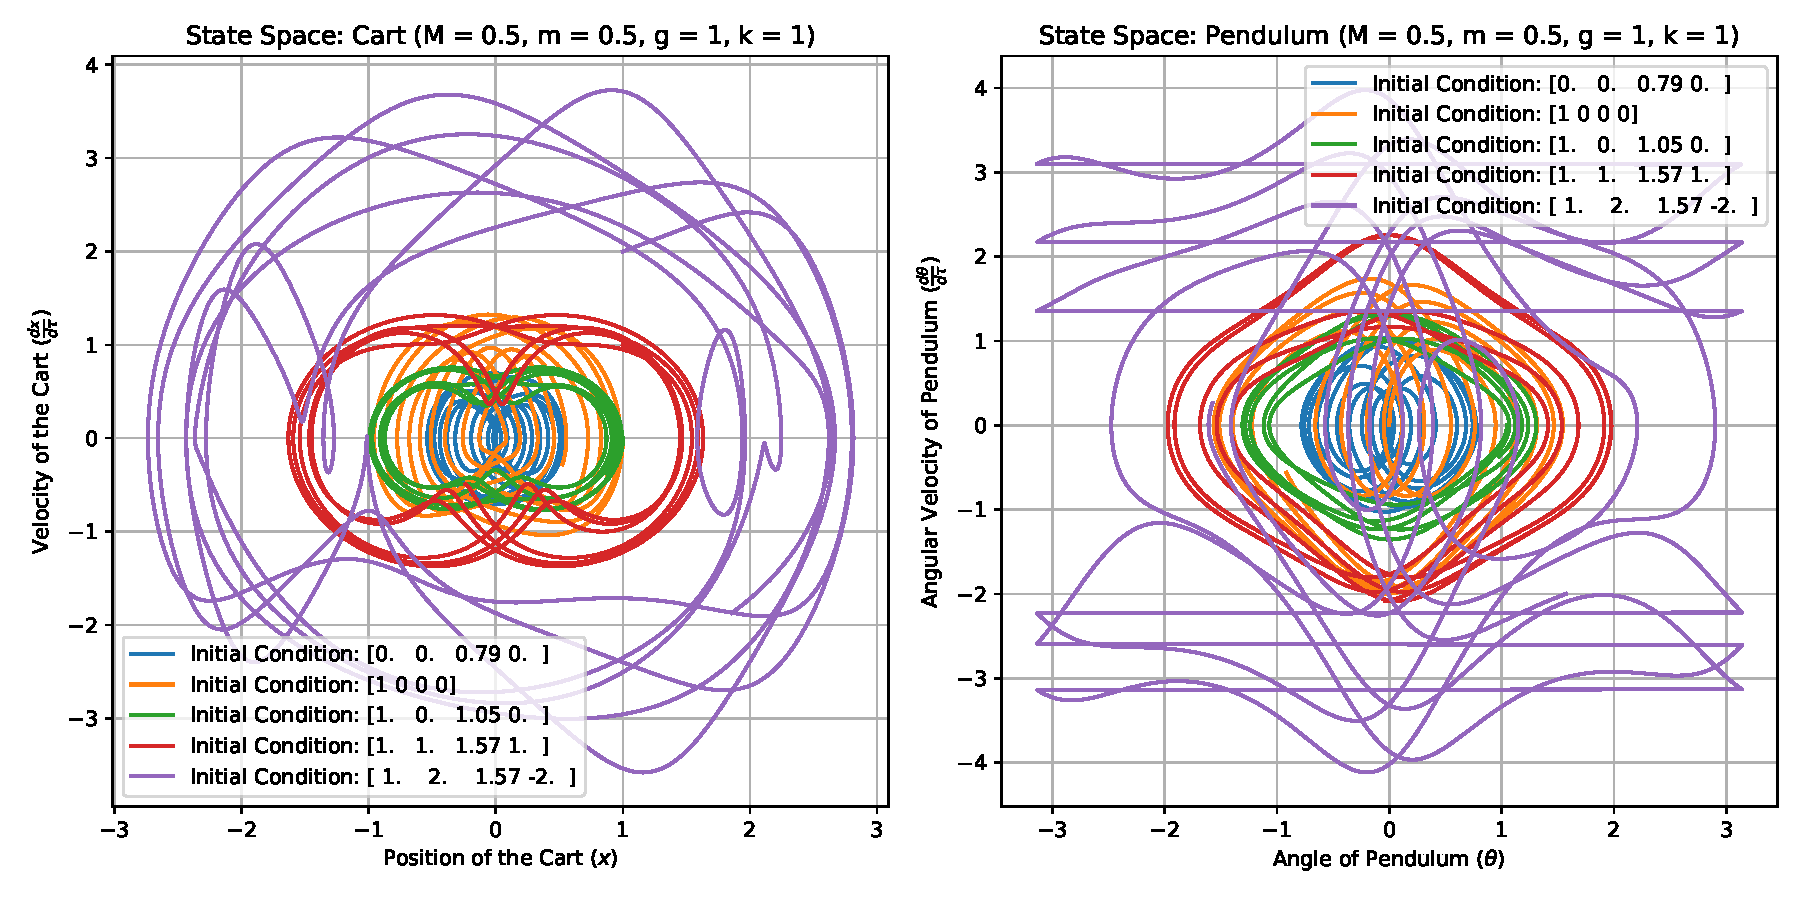
\includegraphics[width=0.9\textwidth]{figures/r-1-k-1-g-1.pdf}} \\
    \subfloat{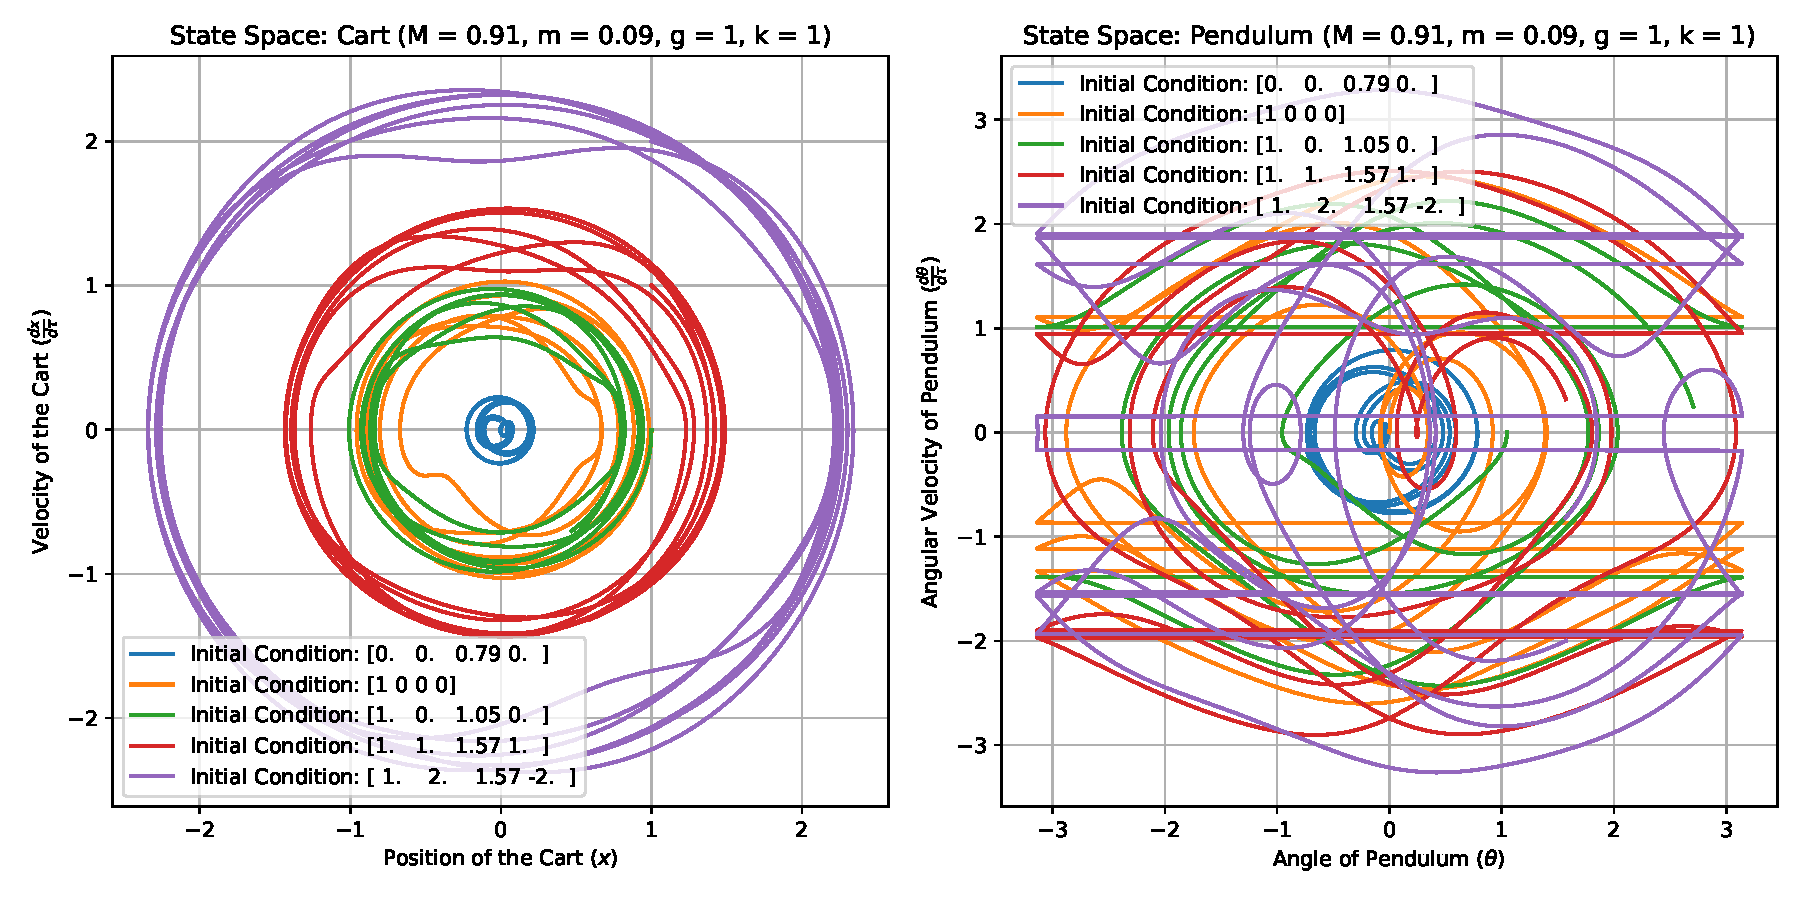
\includegraphics[width=0.9\textwidth]{figures/r-10-k-1-g-1.pdf}}
    \caption{\small{Series of state space plots where $f_{msp} = \ f_{pen}$ ($g$ = 1, $k$ = 1). From top to bottom, the rows illustrate the mass ratios 0.1, 1, and 10. On the left is the state space of $X$ and that of $\theta$ on the right. The initial conditions are ordered as $[X_0, \frac{dX}{d\tau}_0, \theta_0, \frac{d\theta}{d\tau}_0]$.}}
    \label{fig:mixed-mode}
\end{figure}

\section{Conclusion}
We found that the natural angular frequencies could be used as an indicator for stability analysis of the sub-systems: mass spring system and pendulum. In our exploration, the sub-system with a greater natural angular frequency tends to possess a higher level of stability. Moreover, in the mass spring system, the stability could be further reinforced by increasing its mass compared to the pendulum. This could be explained by the physical limitation of the mass spring system, as it cannot wrap around itself like the pendulum system, where the angle repeats after it exceeds $[-\pi, \pi]$. Lastly, since the energy is conserved in our system, we found out that the initial conditions where the stored energy is higher has a greater chance of driving the overall system into chaotic motion.

To further understand the system, a different system parameters variation scheme should be meaningful. In our study, we chose to vary the natural angular frequency of the pendulum by changing $g$, resulting in a high potential barrier where the pendulum could not flip around itself. However, the length of the pendulum $l$ is another free parameter that could be studied in concurrent with other parameters like the spring constant $k$ and the two masses $M$ and $m$ to examine different scenarios that would grant a deeper understanding of the overall system.

All of the code we used for the project can be found on GitHub \href{https://github.com/NextZtepS/SpringedCart_and_Pendulum/tree/main}{here}.

\end{document}
